\chapter{Background}
\vspace{1cm}

Background blah.

\section{File Systems}

\todo{Find reference for basic file system stuff.}

The file system is a fundamental abstraction for almost all modern operating
systems. The abstraction allows the operating system and user programs to
interact with a variety of devices and services through a single unified
interface.
The purpose of a specific file system is to implement this common interface for
a particular underlying data store. The exact nature of the data store is not
important to the consumer of the file system's interface. The underlying data
store is commonly a physical storage device such as a hard disk drive (HDD).
However, it is important to note that this is not always the case and there is
no requirement for a file system to manage a physical storage device. File
systems that depend on another file system as their underlying data store are
known as a VFS (virtual file system).

The high level filing cabinet metaphor that is built on the low level interface
provided by a particular file system implementation will be familiar to most
computer users. The metaphor consists of a filing cabinet containing many named
files. These files can contain arbitrary data. However, some of these files may
not contain data themselves but rather other files, and in this case they are
called directories (or folders in some versions of the metaphor). This nesting
of files within directories creates a hierarchical structure where a single
root directory (analogous to the filing cabinet) contains an arbitrarily
deeply nested series of files and directories. The hierarchy of files within
directories can conceptually be arbitrarily deep, but most particular
implementations enforce a limit for simplicity. The filing cabinet metaphor is
also useful in demonstrating that a file or directory can only be contained
within one other directory. Each file or directory (excluding the root
directory) must have one and only one parent in the hierarchy.

In Figure~\ref{fig:sample file hierarchy} there are two distinct files named
\texttt{timeline.txt}. It becomes ambiguous to refer to a file only by its name
when this is the case. It is useful to use the steps taken to arrive at a file
or directory to identify it within the file hierarchy. For example, the steps
taken to arrive at \texttt{timeline.txt} would be \texttt{/} then
\texttt{documents} then \texttt{project1} then \texttt{timeline.txt}. This list
of steps is known as a path and can be written as a \texttt{/} delimited list
of the steps taken to reach a file or directory. Using the previous example the
path would be \texttt{/documents/project1/timeline.txt}. As a result of the
single parent rule, each file or directory has a single path that uniquely
identifies it amongst all other files and directories in the hierarchy. This
single unique path is known as an absolute path, meaning the steps to arrive at
a file or directory are completely specified all the way from the root of the
file system\footnote{This is not the case when the file system contains
symbolic links.}. In contrast to this, a relative path is a path that is not
specified from the root of the file system, but from some other arbitrary
location. For example, the path \texttt{project1/timeline.txt} is a relative
path that is specified from the \texttt{documents} directory. The directory
that a relative path is specified from is known as the current working
directory.

The strict hierarchical nature of the file system falls apart with the addition
of links to the file system. There are two types of links in UNIX file systems:
hard links and symbolic (or soft) links. Symbolic links (often abbreviated as
symlinks) are a special kind of file-like object that act as a window into
another part of the file system. Symbolic links have a name like a normal file,
but they additionally have a target which is another path that they act as a
window into. For example, you could imagine a symbolic link named
\texttt{my-link} in the \texttt{images} directory with a target of
\texttt{/code}. The existence of this link would mean that now the path
\texttt{/images/my-link/main.c} refers to the same file as
\texttt{/code/main.c} (the same property holds for
\texttt{/images/my-link/Makefile} also). \todo{Talk about how symbolic links
can introduce cycles.}

A hard link is a reference to a piece of data. Hard links are very similar to
regular files, because regular files are in fact hard links. A hard link
references an inode\footnote{\todo{Explain that even Dennis Ritchie does not
know exactly why an inode is called an inode.}
https://lkml.indiana.edu/hypermail/linux/kernel/0207.2/1182.html} \cite{inode}
by way of an inode number. An inode is a data structure internal to the file
system that is used to keep track of metadata relating to some user data. An
inode number is a number that uniquely identifies an inode on a particular file
system. The consequence of this is that hard links, and therefore regular
files, don't actually own their data; they only reference it through an inode
number. This means that there can be multiple distinct files that reference the
same inode, and therefore are associated with the same data.

% Sample file hierarchy figure {{{
\begin{figure}[h]
\centering
\begin{forest}
    for tree = {%
        folder,
        grow'=0,
        fit=band,
        font=\ttfamily,
        s sep=0.5mm,
        l sep=0.7cm,
    }
    [/,color=teal
        [code,color=teal
            [main.c,color=olive]
            [Makefile,color=olive]
        ]
        [documents,color=teal
            [project1,color=teal
                [timeline.txt,color=olive]
            ]
            [project2,color=teal
                [timeline.txt,color=olive]
            ]
            [projects.txt,color=olive]
        ]
        [images,color=teal
            [scan.jpg,color=olive]
        ]
    ]
\end{forest}
\caption[Sample file hierarchy]{Sample file hierarchy with directories in
    \textcolor{teal}{blue}
    and files in \textcolor{olive}{green}.}
\label{fig:sample file hierarchy}
\end{figure}
% }}}

\subsection{Operating Systems and the File System}

\todo{
    Talk about how ls makes a system call and the kernel receives it and then
    calls the fuse kernel module who then writes to unix socket which fuser
    (Rust) reads who then calls me. In the general case libFUSE would call the
    libc function mount with fs type 'fuse'. In my case fuser calls fusermount3
    and listens to the returned unix socket for messages from the kernel.
}

The primary way most users interact with file systems is through a GUI
(graphical user interface) file manager such as \texttt{thunar} or
\texttt{nautilus}. \todo{Maybe screenshot of file manager with tree view?}
However, it is also possible to manage a file system without a GUI and use CLI
(command line interface) tools such as \texttt{ls} or \texttt{mv}. Both GUI
file managers and CLI tools utilise the low level interface exposed by the
operating system and implemented by a particular file system. The traditional
way to use this interface is via the platform library exposed by the operating
system\footnote{On some platform like Microsoft Windows, using the platform
library is required because the system call interface is not guaranteed to be
stable between releases.}. \todo{Not sure if I should stay abstract about a
particular operating system or be specifically about UNIX-likes here.} On
UNIX-like operating systems this library is \texttt{libc} \cite{libc}. \todo{Do
I need to talk about the difference between an abstract libc and concrete like
glibc or musl?} The overwhelming majority of programs that run on UNIX-like
operating systems use \texttt{libc} to help them interact with the platform.
The operating systems' \texttt{libc} contains functions that require access to
the file system (such as \texttt{stat} \cite{stat-syscall}). To get access to
the file system the \texttt{libc} function will execute a system
call \cite{syscalls} (often called a syscall). A system call is a way for an
unprivileged user program to ask the operating system to perform an action on
its behalf. When executed, a system call performs a context switch
\todo{Explain what a context switch actually is.} and jumps into kernel
code\footnote{This is not strictly true, some system calls do not require
jumping into kernel code.}. The kernel is the part of the operating system
that, amongst many other functions, responds to system calls. When the kernel
responds to a system call that requires accessing the file system, it must
first ascertain which file system implementation is the correct one to call for
this particular action. On Linux this is the VFS layer in the kernel
\cite{kernel-vfs}. Once this is determined, the kernel asks the file system
implementation to perform the action specified by the system call. It may also
return some data to the calling user program via a buffer or a return value.

\subsection{FUSE File Systems}

% FUSE diagram figure {{{
\begin{figure}[h]
    \centering
    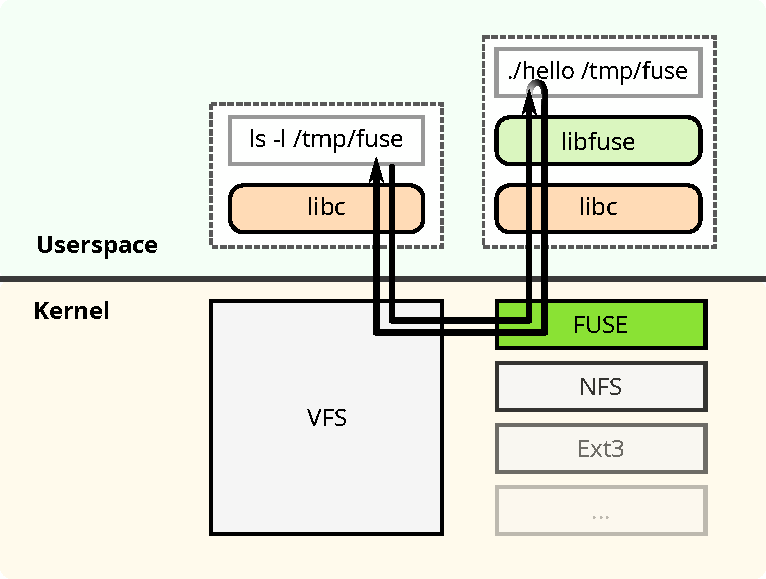
\includegraphics[width=10cm]{../data/fuse.pdf}
    \caption[FUSE Data Flow]{A diagram to show the flow of data in a FUSE file
        system. Taken from \cite{fuse-diagram-source}}
    \label{fig:fuse diagram}
\end{figure}
% }}}

Most file systems are built into the kernel; either directly compiled in or as
kernel modules. This means they will run in kernel mode (ring 0 on x86
platforms). If code running as part of the kernel crashes or hangs, there is a
danger that this could crash or hang the entire system. Additionally, code
running in kernel mode has the power to do anything on the system, so a
security issue in any code run at this level code could result in a compromised
system. To reduce the danger of writing a file system, Linux allows file
systems to be run as userspace processes using a technology called
FUSE \cite{kernel-fuse} (file system in userspace).

Looking at Figure~\ref{fig:fuse diagram}, there are similarities between the
process of accessing a file system built into the kernel (in the diagram NFS
and ext3 are used as an example) and the process of accessing a FUSE file
system. For both built in file systems and FUSE file systems, the calling
program uses \texttt{libc} to ask the kernel to perform a file system action,
and the kernel dispatches the call to the correct file system implementation
using the VFS layer. When the VFS layer requires action from a FUSE file
system, it passes the request to the FUSE kernel module. The FUSE kernel module
then communicates (the nature of the communication and the medium across which
it takes place are discussed in Section~\ref{mounting-fuse-fs}) the request to
the user space process. The user space process can then do whatever it pleases
to generate a response which is then passed back through the layers into the
kernel and back to the calling user space program that made the request.

FUSE file systems provide more flexibility and safety compared to file systems
compiled into the kernel. However, this flexibility comes at performance and
hardware utilisation cost with an average of a 31\% increase in CPU utilisation
when file system requests are routed through the FUSE layer \cite{fuse-perf}.
The performance decrease has a larger variance with some cases having as low as
5\% overhead. However, in other cases that are "unfriendly to FUSE" such as
concurrent random access to large files can cause an 83\% decrease in
performance even if optimised \cite{fuse-perf}.

\subsubsection{Mounting FUSE File Systems}
\label{mounting-fuse-fs}

To mount a (non-root) file system means attaching the root of a child file
system to an empty directory in another parent file system. The two file
systems remain entirely independent; their connection is only simulated using
the kernel's VFS layer. However, to other programs it appears that the contents
of the child file system are available as a sub-directory in another parent
file system. This allows the composition of many independent file systems into
one virtual file system with the kernel handling dispatching requests to the
correct underlying file system.

On Linux mounting a file system is a restricted operation that can only be
performed by the root user \cite{mount}. However, FUSE has the explicit goal of
"allowing secure, non-privileged mounts" \cite{kernel-fuse}. To allow FUSE file
systems to be mounted by non-privileged users, FUSE provides a mounting utility
\texttt{fusermount} which is installed with the setuid \cite{setuid} permission
set to the root user. A binary with this permission can be run by a normal
user, but whilst it is running it has all the privileges of the root user. This
allows a normal user to mount a FUSE file system.

After the FUSE file system has been mounted there needs to be a channel for
communication between the FUSE kernel module and the user space program
managing the file system. This channel is the \texttt{/dev/fuse} pseudo device
file. However, reading and writing to this file is a privileged action so
\texttt{fusermount} (with its elevated permissions) is responsible for opening
a handle to \texttt{/dev/fuse} and then returning it to the user space file
system. \texttt{fusermount} returns this handle over a socket given to it via
an environment variable at launch.

\todo{Talk (briefly I think) about the binary protocol fuse talks over
\texttt{/dev/fuse}}

\section{Memory Safety and the Rust Programming Language}

In this section I will attempt to give a brief overview of the Rust programming
language and how it ensures memory safety without the use of a runtime garbage
collector. Also I will talk about why memory safety is important, and the
problems caused when it is not adhered to.

Memory safety is a property of a program that means that the program does not
under any circumstances have any bugs relating to invalid pointer access or
accessing uninitialised data \todo{source?}. These two classes of bug contain
many common sources of security issues in programs such as use-after-free,
buffer overflow, and invalid pointer dereferences. In fact memory safety
related bugs are some of the most frequent security bugs in many widely used
software packages such as Chromium \cite{chromium-mem-safety}, with the project
estimating that 70\% of their security bugs are related to memory safety
issues.

\todo{Talk about and define exactly what are use-after-free, buffer overflow
etc.}
\todo{Talk about how memory leaks are not a memory safety issue.}

One way of ensuring memory safety is through the use of a runtime garbage
collector. This, in addition to disallowing pointer arithmetic, ensures memory
safety by not allowing the user program to directly allocate and free memory
itself, and by not allowing access to invalid memory locations. However, for
some programs runtime garbage collection is not suitable for performance
reasons. For example, real time systems with hard deadlines may not be able to
use a garbage collector due to the unpredictability of the moment of and the
duration of garbage collection pauses. It is in these case where a language
like Rust can prove its value by having fast and consistent performance as well
as memory safety.

Rust ensures memory safety by refusing to compile programs that do not satisfy
a particular set of rules at compile time. The sub-system in the Rust compiler
that checks these rules against the given code is called the ``borrow
checker''. The borrow checker works via the concept of ``ownership''
\cite{rust-book-ownership}. Ownership means that every value in a Rust program
has one and only one owner. When the owner is no longer accessible i.e. it has
gone out of scope, then the value it owns is freed (or in Rust parlance
``dropped''). Ownership of a value can be transferred or handed over to another
owner, but once this has occurred the original owner is unable to access the
value therefore preserving the single owner rule. Ensuring that a value only
has one owner in this way is enough to be able to statically insert calls to
free values when they go out of scope. Transferring ownership of a value can be
cumbersome when it is only temporary, to reduce the burden of always
transferring ownership Rust has the concept of ``borrowing'' a value and
receiving a ``reference'' to it. A reference is similar to a pointer in other
languages, but it is additionally constrained by the fact that all references
must always be valid at all times. Valid meaning that the pointer is not null
and that the pointer has not been freed or deallocated. There are two types of
reference in Rust: mutable and immutable. To ensure memory safety Rust enforces
the rules that there can be either one mutable reference or many immutable
references at any given time, but never both.

An example of memory unsafe code that Rust prevents is shown in
Figure~\ref{fig:rust-xor-borrow-rule}. In the first line a vector is allocated
and initialised with the values 1, 2, and 3. The vector is given the name
``data'' and prefixed with the ``mut'' modifier to state that this value is
allowed to be mutated (in Rust values are immutable by default). In the second
line we borrow from the vector to obtain an immutable reference to the first
item in the vector and then store the reference in the ``first'' variable. Then
on the third line the value 4 is pushed onto the end of the vector. The
``push'' method requires mutable access to the vector to perform its
modification to the vector\footnote{We can see this explicitly in the type
signature of the ``push'' method on vectors ``\texttt{pub fn push(\&mut self,
value: T)}''. The key is the ``mut'' keyword after the \texttt{\&} to indicate
a mutable reference is required.}. On the final line, the reference stored in
the ``first'' variable is used to access the first value of the vector and
print it out. This code is disallowed by the Rust compiler because, on the
third line, the code attempts to acquire a mutable reference to the data vector
whilst an immutable reference is already held, thereby breaking the rules of
the borrow checker.

Additionally, one of the reasons for the enforcement of the ``mutable xor
immutable'' reference rule is illustrated well by the example in
Figure~\ref{fig:rust-xor-borrow-rule}. If this code were allowed to compile
then, in certain situations, the code could attempt to read data from memory
that has been freed. This situation could occur if upon pushing to the vector,
there is no more space in the block of memory underlying the vector. Then to
make more space for the new element, it becomes necessary to grow the vector by
allocating a new larger chunk of memory and copying the existing elements to
the new memory. After the reallocation, the old chunk of memory is freed and
potentially released to the operating system. Now after the push call
completes, the reference held by the ``first'' variable is still pointing to
the location of the old memory allocation which has been freed. When the
reference stored in ``first'' is dereferenced it could cause a segmentation
fault or more insidiously it could only sometimes cause a segmentation fault,
making it very difficult to debug. This is an example of a use-after-free bug,
and one of the ways that Rust prevents them. Interestingly, the code compiles
and runs correctly if the last line is removed. This is because the Rust
compiler is clever enough to be able to notice that the reference stored in the
``first'' variable is not used on or after the third line. Therefore, it is
able to drop the borrow before the third line thereby allowing the mutable
borrow to take place on line three as there are no other references to the
``data'' vector at that time.

% exclusive reference safety example {{{
\begin{figure}[h]
    \centering
    \begin{boxedverbatim}


1 | let mut data = vec![1, 2, 3];
2 | let first = &data[0];

3 | data.push(4);
4 | println!("The first element is: {first}");

-----------------------------------------------
error[E0502]: cannot borrow `data` as mutable because it is also borrowed as immutable
let first = &data[0];
             ---- immutable borrow occurs here

data.push(4);
^^^^^^^^^^^^ mutable borrow occurs here
println!("The first element is: {first}");
                                 ----- immutable borrow later used here
    \end{boxedverbatim}
    \caption[Example of memory unsafe code prevented by Rust]{Example memory
    unsafe code disallowed by Rust's borrow checker with corresponding error
    message}
    \label{fig:rust-xor-borrow-rule}
\end{figure}
% }}}
